\documentclass[aspectratio=169]{beamer}

\usetheme{Boadilla}
\usecolortheme{default}
\setbeamertemplate{navigation symbols}{}
\setbeamertemplate{footline}[frame number]
\setbeamercolor{structure}{fg=teal!70!black}
\setbeamercolor{title}{fg=teal!70!black}
\setbeamercolor{block title}{fg=white,bg=teal!70!black}
\setbeamercolor{block body}{bg=teal!5}

\usepackage{graphicx}
\graphicspath{{docs/images/}}

\title[Crux]{Crux: Video-Based Bouldering Analysis}
\subtitle{Turning climbing footage into interpretable movement cues}
\date{10-minute project presentation}

\begin{document}

% 0:30
\begin{frame}
  \titlepage
\end{frame}

% 1:15
\begin{frame}{Motivation: make practice easier to review}
  \begin{itemize}
    \item A climbing video preserves a move, but it does not explain which
      holds were used or how the climber moved between them.
    \item Reviewing every frame manually can make it difficult to notice
      repeated movement patterns.
    \item We wanted to explore whether computer vision could turn ordinary,
      fixed-camera footage into a useful post-session review aid.
  \end{itemize}
  \vspace{0.5em}
  \begin{block}{The problem we address}
    How can we automatically summarize visible holds, body pose, and a few
    understandable movement cues from a climbing video?
  \end{block}
\end{frame}

% 1:00
\begin{frame}{What is Crux?}
  \begin{columns}[T,onlytextwidth]
    \column{0.52\textwidth}
      Crux is a computer-vision program for reviewing bouldering videos.
      \vspace{0.5em}
      \begin{enumerate}
        \item Select a video recorded with a fixed view of the wall.
        \item Detect the holds and estimate the climber's pose.
        \item Review an annotated video and export the result.
      \end{enumerate}
      \vspace{0.4em}
      It can be run through a desktop app or a command-line interface.
    \column{0.46\textwidth}
      \centering
      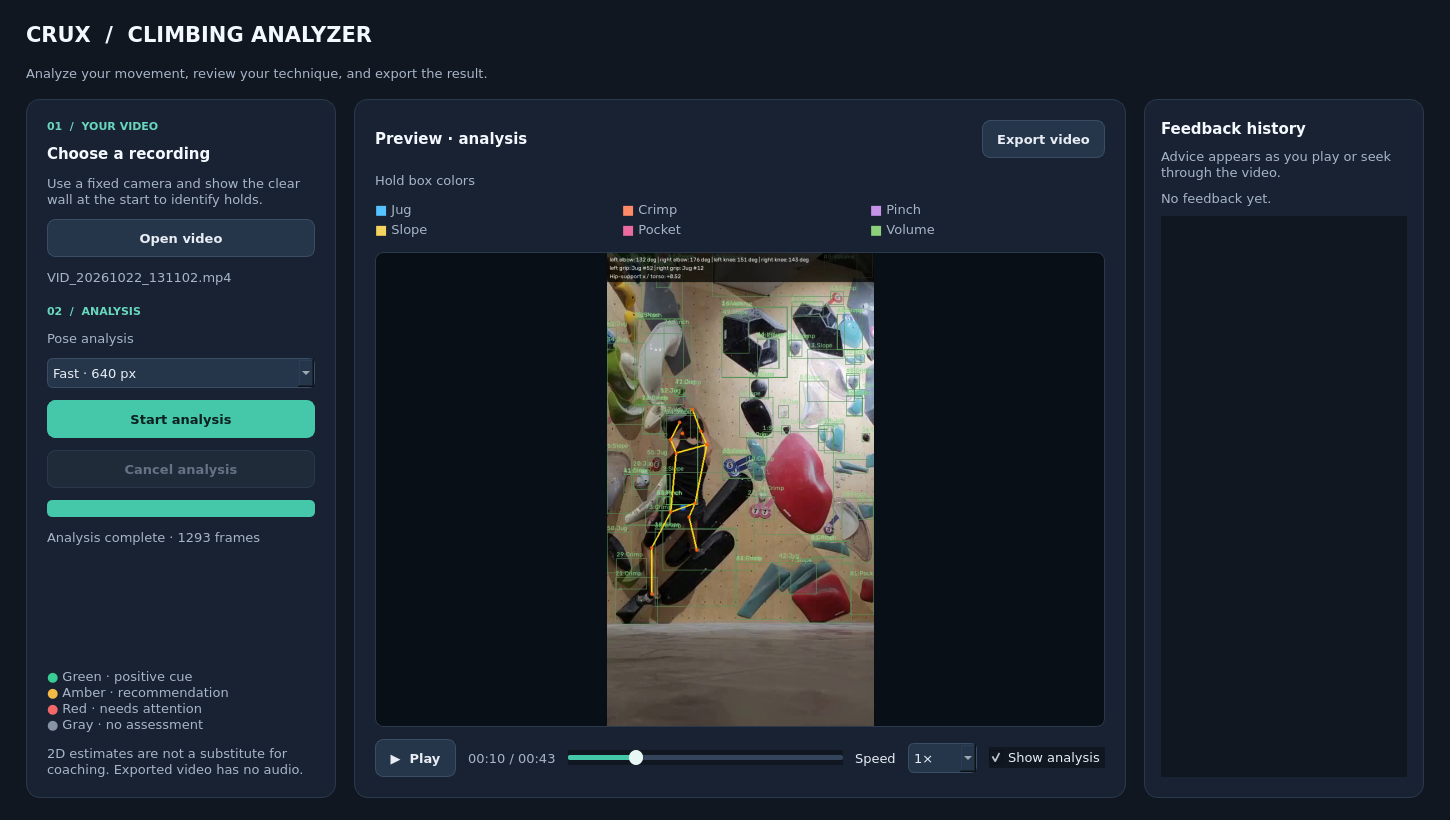
\includegraphics[width=\linewidth,height=0.61\textheight,keepaspectratio]
        {desktop-app.png}
  \end{columns}
\end{frame}

% 1:00
\begin{frame}{Data: teaching the detector what a hold looks like}
  \begin{columns}[T,onlytextwidth]
    \column{0.62\textwidth}
      \begin{itemize}
        \item We use the Indoor Climbing Gym Hold Classification dataset.
        \item Its labeled images contain six hold categories:
          \textbf{Crimp, Jug, Pinch, Pocket, Slope, and Volume}.
        \item Training and validation data support model learning and
          selection; a separate test split is used for evaluation.
        \item The held-out test split contains \textbf{213 images} and
          \textbf{4,677 labeled holds}.
      \end{itemize}
    \column{0.34\textwidth}
      \begin{block}{Important distinction}
        The test split is held out from training, but it comes from the same
        dataset. It does not by itself establish performance in new gyms.
      \end{block}
  \end{columns}
  \vfill
  {\tiny Dataset: Indoor Climbing Gym Hold Classification, linked in the
  project README.}
\end{frame}

% 1:30
\begin{frame}{AI models: two different vision tasks}
  \begin{columns}[T,onlytextwidth]
    \column{0.48\textwidth}
      \begin{block}{Hold detection}
        An Ultralytics YOLO object detector finds hold bounding boxes and
        assigns one of the six categories. The training script uses YOLO
        weights and saves the best checkpoint.
      \end{block}
      \begin{block}{Human pose estimation}
        A YOLOv8m-pose model estimates body keypoints, including shoulders,
        elbows, wrists, hips, knees, and ankles.
      \end{block}
    \column{0.48\textwidth}
      \begin{block}{Video pipeline}
        \centering
        Fixed-camera video\\[0.35em]
        $\Downarrow$\\[0.35em]
        Map holds from the first 15 frames\\[0.35em]
        $\Downarrow$\\[0.35em]
        Estimate pose frame by frame\\[0.35em]
        $\Downarrow$\\[0.35em]
        Annotated video and review cues
      \end{block}
      \small
      The two models provide visual estimates; the coaching layer combines
      them with transparent, hand-written rules.
  \end{columns}
\end{frame}

% 1:15
\begin{frame}{From detections to feedback}
  \begin{itemize}
    \item Pose keypoints are confidence-checked and smoothed over time.
    \item A wrist is associated with a detected hold when it is close to the
      hold box, using torso length to scale the tolerance.
    \item The program estimates joint angles and compares the hip position
      with visible ankle positions as a rough balance proxy.
    \item Simple rules generate category-specific cues. Cues must persist
      before appearing, which reduces flicker in the video.
  \end{itemize}
  \vspace{0.4em}
  \begin{alertblock}{These are estimates, not ground truth}
    Wrist proximity does not prove contact, and visible ankles do not prove
    that a foot is supporting the climber.
  \end{alertblock}
\end{frame}

% 1:15
\begin{frame}{Results: a promising detector on the held-out split}
  \begin{columns}[T,onlytextwidth]
    \column{0.46\textwidth}
      \begin{block}{Hold-detector test results}
        \begin{itemize}
          \item Precision: \textbf{95.1\%}
          \item Recall: \textbf{93.4\%}
          \item mAP@0.50: \textbf{96.4\%}
          \item mAP@0.50:0.95: \textbf{91.7\%}
        \end{itemize}
      \end{block}
      \small
      One evaluation on 213 test images with 4,677 labeled holds. These
      numbers evaluate hold detection, not the accuracy or usefulness of
      coaching cues.
    \column{0.51\textwidth}
      \centering
      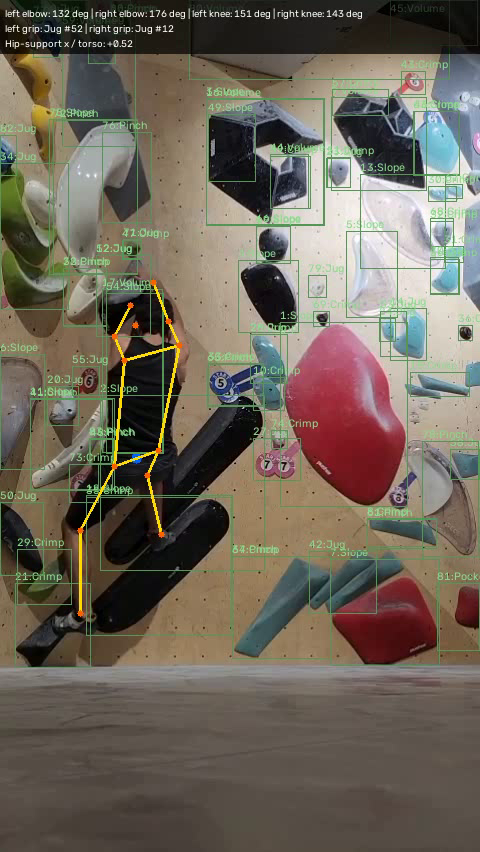
\includegraphics[width=\linewidth,height=0.62\textheight,keepaspectratio]
        {analyzed-result-wall-1.png}
  \end{columns}
\end{frame}

% 1:15
\begin{frame}{Potential impact and current limitations}
  \begin{columns}[T,onlytextwidth]
    \column{0.48\textwidth}
      \begin{block}{Potential value}
        \begin{itemize}
          \item Make video review more structured.
          \item Help climbers revisit visible movement patterns after a
            session.
          \item Offer a starting point for discussion with a human coach.
        \end{itemize}
        These are intended uses, not outcomes established by a user study.
      \end{block}
    \column{0.48\textwidth}
      \begin{alertblock}{Limitations}
        \begin{itemize}
          \item Designed for a fixed, clear camera view.
          \item Uses 2D image-space estimates, not true contact or center of
            mass.
          \item Can be affected by occlusion, camera motion, or multiple
            climbers.
          \item Not professional coaching, a diagnosis, or a safety
            assessment.
        \end{itemize}
      \end{alertblock}
  \end{columns}
\end{frame}

% 1:00
\begin{frame}{Conclusion}
  \begin{itemize}
    \item Crux combines hold detection and pose estimation to annotate
      fixed-camera bouldering videos.
    \item Its detector achieved strong results on one held-out split, while
      the movement feedback remains an experimental 2D heuristic.
    \item The project addresses a practical review problem without claiming
      to replace a coach or verify safe technique.
  \end{itemize}
  \vspace{0.7em}
  \begin{block}{Next step}
    Evaluate videos from more gyms, camera setups, and climbers, then compare
    the generated cues with expert feedback.
  \end{block}
  \centering
  \vspace{0.5em}
  \Large Thank you
\end{frame}

\end{document}
